\documentclass[a4paper, 12pt]{article}

\usepackage{arxiv}

\usepackage[T2A]{fontenc}
\usepackage[utf8]{inputenc}
\usepackage[english, russian]{babel}
% \usepackage{cmap}
\usepackage{url}
\usepackage{booktabs}
\usepackage{nicefrac}
\usepackage{microtype}
\usepackage{lipsum}
\usepackage{graphicx}
\usepackage{subfig}
\usepackage[square,sort,comma,numbers]{natbib}
\usepackage{doi}
\usepackage{multicol}
\usepackage{multirow}
\usepackage{tabularx}

\usepackage{tikz}
\usetikzlibrary{matrix}

% Algorithms
\usepackage{algpseudocode}
\usepackage{algorithm}

%% Шрифты
\usepackage{euscript} % Шрифт Евклид
\usepackage{mathrsfs} % Красивый матшрифт
\usepackage{extsizes}

\usepackage{makecell} % diaghead in a table
\usepackage{amsmath,amsfonts,amssymb,amsthm,mathtools,dsfont}
\usepackage{icomma}

\usepackage{hyperref}
% \usepackage[usenames,dvipsnames,svgnames,table,rgb]{xcolor}

\hypersetup{
	unicode=true,
	pdftitle={Байесовский подход к выбору достаточного размера выборки},
	pdfauthor={Киселев Никита Сергеевич},
	pdfkeywords={определение размера выборки, байесовский подход},
	colorlinks=true,
	linkcolor=black,        % внутренние ссылки
	citecolor=green,         % на библиографию
	filecolor=magenta,      % на файлы
	urlcolor=blue           % на URL
}

\graphicspath{{./figures/}}

\usepackage{enumitem} % Для модификаций перечневых окружений
\usepackage{etoolbox}

\makeatletter
\expandafter\patchcmd\csname\string\algorithmic\endcsname{\itemsep\z@}{\itemsep=1.5mm}{}{}
\makeatother

% Теоремы
\newtheorem{theorem}{Теорема}
\newtheorem{lemma}{Лемма}
\newtheorem{proposition}{Утверждение}
\newtheorem*{exercise}{Упражнение}
\newtheorem*{problem}{Задача}

\newtheorem{definition}{Определение}
\newtheorem*{corollary}{Следствие}
\newtheorem*{note}{Замечание}
\newtheorem*{reminder}{Напоминание}
\newtheorem*{example}{Пример}
\newtheorem*{cexample}{Контрпример}
\newtheorem*{solution}{Решение}

\renewcommand{\abstractname}{Аннотация}
% latin bold lower
\newcommand{\ba}{\mathbf{a}} 
\newcommand{\bc}{\mathbf{c}} 
\newcommand{\be}{\mathbf{e}} 
\newcommand{\bh}{\mathbf{h}} 
\newcommand{\bp}{\mathbf{p}} 
\newcommand{\bt}{\mathbf{t}} 
\newcommand{\bs}{\mathbf{s}} 
\newcommand{\bu}{\mathbf{u}} 
\newcommand{\bv}{\mathbf{v}} 
\newcommand{\bw}{\mathbf{w}} 
\newcommand{\bx}{\mathbf{x}} 
\newcommand{\by}{\mathbf{y}} 
\newcommand{\bz}{\mathbf{z}} 

% latin bold upper
\newcommand{\bA}{\mathbf{A}} 
\newcommand{\bB}{\mathbf{B}} 
\newcommand{\bC}{\mathbf{C}} 
\newcommand{\bI}{\mathbf{I}} 
\newcommand{\bJ}{\mathbf{J}} 
\newcommand{\bL}{\mathbf{L}} 
\newcommand{\bM}{\mathbf{M}} 
\newcommand{\bP}{\mathbf{P}}
\newcommand{\bQ}{\mathbf{Q}} 
\newcommand{\bR}{\mathbf{R}} 
\newcommand{\bT}{\mathbf{T}} 
\newcommand{\bU}{\mathbf{U}} 
\newcommand{\bV}{\mathbf{V}} 
\newcommand{\bW}{\mathbf{W}} 
\newcommand{\bX}{\mathbf{X}} 
\newcommand{\bY}{\mathbf{Y}} 
\newcommand{\bZ}{\mathbf{Z}} 

% latin cal upper
\newcommand{\cF}{\mathcal{F}} 
\newcommand{\cG}{\mathcal{G}} 
\newcommand{\cI}{\mathcal{I}} 
\newcommand{\cL}{\mathcal{L}} 
\newcommand{\cM}{\mathcal{M}} 
\newcommand{\cN}{\mathcal{N}} 
\newcommand{\cS}{\mathcal{S}} 
\newcommand{\cT}{\mathcal{T}} 
\newcommand{\cW}{\mathcal{W}} 
\newcommand{\cX}{\mathcal{X}} 
\newcommand{\cZ}{\mathcal{Z}} 

% latin bb upper
\newcommand{\bbE}{\mathbb{E}} 
\newcommand{\bbI}{\mathbb{I}} 
\newcommand{\bbP}{\mathbb{P}} 
\newcommand{\bbR}{\mathbb{R}} 

% greek bold lower
\newcommand{\bepsilon}{\boldsymbol{\epsilon}} 
\newcommand{\btheta}{\boldsymbol{\theta}} 
\newcommand{\blambda}{\boldsymbol{\lambda}} 
\newcommand{\bpi}{\boldsymbol{\pi}} 
\newcommand{\bmu}{\boldsymbol{\mu}} 
\newcommand{\bsigma}{\boldsymbol{\sigma}} 
\newcommand{\bphi}{\boldsymbol{\phi}} 

% greek bold upper
\newcommand{\bSigma}{\boldsymbol{\Sigma}} 

\DeclareMathOperator*{\argmin}{arg\,min}
\DeclareMathOperator*{\argmax}{arg\,max}

\title{Байесовский подход к выбору достаточного размера выборки}

\author{
    Киселев Никита \\
	\texttt{kiselev.ns@phystech.edu} \\
	\And
	Грабовой Андрей \\
	\texttt{grabovoy.av@phystech.edu} \\
}

\date{\today}

\begin{document}

%%% Название
\maketitle

%%% Аннотация
\begin{abstract}
	Исследуется задача выбора достаточного размера выборки. Рассматривается проблема определения достаточного размера выборки без учета природы параметров используемой модели. Предлагается использовать функцию правдоподобия выборки. Используются подходы на основе эвристик о поведении функции правдоподобия при достаточном количестве объектов в выборке. Проводится вычислительный эксперимент для анализа свойств предложенных методов.
\end{abstract}

\keywords{определение размера выборки \and байесовский подход}

%%% Введение
\section{Введение}

Задача машинного обучения с учителем предполагает выбор предсказательной модели из некоторого параметрического семейства. Обычно такой выбор связан с некоторыми статистическими гипотезами, например, максимизацией некоторого функционала качества. 
\begin{definition}
    Модель прогнозирования, которая соответствует этим статистическим гипотезам, называется \textbf{адекватной} моделью.
\end{definition}

При проведении эксперимента зачастую дана конечная обучающая выборка.

\begin{definition}
    Размер выборки, необходимый для построения адекватной модели прогнозирования, называется \textbf{достаточным}.
\end{definition}

В работе \cite{Grabovoy2022} представлены десять методов для оценки достаточного размера выборки. Среди них есть как статистические, так и байесовские подходы. 

%%% Основная часть
\section{Постановка задачи}\label{sec1}

Объектом называется пара $(\bx, y)$, где $\bx \in \mathbb{X} \subseteq \mathbb{R}^n$ есть вектор признакового описания объекта, а $y \in \mathbb{Y}$ есть значение целевой переменной. В задаче регрессии $\mathbb{Y} = \mathbb{R}$, а в задаче $K$-классовой классификации $\mathbb{Y} = \{1, \ldots, K\}$.

Матрицей объекты-признаки для выборки $\mathfrak{D}_m = \left\{ (\bx_i, y_i) \right\}, i \in \mathcal{I} = \{ 1, \ldots, m \}$ размера $m$ называется матрица $\bX = \left[ \bx_1, \ldots, \bx_m \right]\T \in \mathbb{R}^{m \times n}$.

Вектором ответов (вектором значений целевой переменной) для выборки $\mathfrak{D}_m = \left\{ (\bx_i, y_i) \right\}, i \in \mathcal{I} = \{ 1, \ldots, m \}$ размера $m$ называется вектор $\by = \left[ y_1, \ldots, y_m \right]\T \in \mathbb{Y}^m$.

Моделью называется параметрическое семейство функций $f$, отображающих декартово произведение множества значений признакового описания объектов $\mathbb{X}$ и множества значений параметров $\mathbb{W}$ во множество значений целевой переменной $\mathbb{Y}$: $$f: \mathbb{X} \times \mathbb{W} \to \mathbb{Y}.$$

Вероятностной моделью называется совместное распределение вида $$p(y, \bw | \bx) = p(y | \bx, \bw) p(\bw): \mathbb{Y} \times \mathbb{W} \times \mathbb{X} \to \mathbb{R}^+,$$
где $\bw \in \mathbb{W}$ есть набор параметров модели, $p(y | \bx, \bw)$ задает правдоподобие объекта, а $p(\bw)$ задает априорное распределение параметров.

Функцией правдоподобия простой выборки $\mathfrak{D}_m = \left\{ (\bx_i, y_i) \right\}, i \in \mathcal{I} = \{ 1, \ldots, m \}$ размера $m$ называется функция $$L(\mathfrak{D}_m, \mathbf{w}) = p(\by | \bX, \bw) = \prod_{i=1}^{m} p(y_i | \mathbf{x}_i, \mathbf{w}).$$ Ее логарифм $$l(\mathfrak{D}_m, \mathbf{w}) = \sum\limits_{i=1}^{m} \log p(y_i | \mathbf{x}_i, \mathbf{w})$$ называется логарифмической функцией правдоподобия. Далее, если не оговорено противное, будем считать выборку простой.

Оценкой максимума правдоподобия набора параметров $\bw \in \mathbb{W}$ по выборке $\mathfrak{D}_m = \left\{ (\bx_i, y_i) \right\}, i \in \mathcal{I} = \{ 1, \ldots, m \}$ размера $m$ называется $$\hat{\mathbf{w}}_{m} = \argmax_{\bw \in \mathbb{W}} L(\mathfrak{D}_m, \mathbf{w}).$$

Ставится задача определения достаточного размера выборки $m^*$. Пусть задан некоторый критерий $T$. Он может быть построен, например, на основе эвристик о поведении параметров модели.
\begin{definition}
    Размер выборки $m^*$ называется \textbf{достаточным} согласно критерию $T$, если $T$ выполняется для всех $k \geqslant m^*$.
\end{definition}
Стоит учесть, что возможно $m^* \leqslant m$ или $m^* > m$. Эти два случая будут отдельно рассмотрены далее.
\section{Достаточный размер выборки не превосходит доступный}\label{sec2}

В этой главе будем считать, что достоверно $m^* \leqslant m$.

Рассмотрим выборку $\mathfrak{D}_k$ размера $k \leqslant m$. Оценим на ней параметры, используя метод максимума правдоподобия:
\[ \hat{\mathbf{w}}_{k} = \arg\max_{\mathbf{w}} L(\mathfrak{D}_k, \mathbf{w}). \]

Поскольку природа $\mathbf{w}$ нам неизвестна, для определения достаточности будем использовать функцию правдоподобия.

Когда в наличии имеется достаточно объектов, вполне естественно ожидать, что от одной реализации выборки к другой полученная оценка параметров не будет сильно меняться \cite{Joseph1997, Joseph1995}. То же можно сказать и про функцию правдоподобие. Таким образом, сформулируем, какой размер выборки можно считать достаточным.

\begin{definition}
    \label{sufficient-variance}
    Зафиксируем некоторое положительное число $\varepsilon > 0$. Размер выборки $m^*$ называется \textbf{D-достаточным}, если для любого $k \geqslant m^*$
    \[ D(k) = \mathbb{D}_{\mathfrak{D}_k} L(\mathfrak{D}_m, \hat{\mathbf{w}}_{k}) \leqslant \varepsilon. \]
\end{definition}
\begin{note}
    В определении~\ref{sufficient-variance} вместо функции правдоподобия $L(\mathfrak{D}_m, \hat{\mathbf{w}}_{k})$ можно рассматривать ее логарифм $l(\mathfrak{D}_m, \hat{\mathbf{w}}_{k})$.
\end{note}

С другой стороны, когда в наличии имеется достаточно объектов, также вполне естественно, что при добавлении очередного объекта в рассмотрение полученная оценка параметров не будет сильно меняться. Сформулируем еще одно определение.

\begin{definition}
    \label{sufficient-difference}
    Зафиксируем некоторое положительное число $\varepsilon > 0$. Размер выборки $m^*$ называется \textbf{M-достаточным}, если для любого $k \geqslant m^*$ 
    \[ M(k) = \left| \mathbb{E}_{\mathfrak{D}_{k+1}} L(\mathfrak{D}_m, \hat{\mathbf{w}}_{k+1}) - \mathbb{E}_{\mathfrak{D}_k} L(\mathfrak{D}_m, \hat{\mathbf{w}}_{k}) \right| \leqslant \varepsilon. \]
\end{definition}
\begin{note}
    В определении~\ref{sufficient-difference} вместо функции правдоподобия $L(\mathfrak{D}_m, \hat{\mathbf{w}}_{k})$ можно рассматривать ее логарифм $l(\mathfrak{D}_m, \hat{\mathbf{w}}_{k})$.
\end{note}

\textcolor{red}{Как доказать корректность этих определений? А именно, почему такой размер выборки существует?}

Предположим, что $\mathbb{W} = \mathbb{R}^n$, т.е. параметры $\bw$ представляются в виде вектора. Напомним, что информацией Фишера называется матрица
\[ \left[\mathcal{I}(\bw)\right]_{ij} = - \mathbb{E}\left[ \dfrac{\partial^2 \log p(\by | \bX, \bw)}{\partial w_i \partial w_j} \right]. \]
Достаточно известным результатом является асимптотическая нормальность оценки максимума правдоподобия. 

\begin{proposition}
    Пусть $\hat{\bw}_k$~--- оценка максимума правдоподобия $\bw$. Тогда при определенных условиях регулярности (которые на практике чаще всего выполнены) имеет место следующая сходимость по распределению:
    \[ \sqrt{m}\left( \hat{\bw}_k - \bw \right) \xrightarrow{d} \mathcal{N}\left(0, \mathcal{I}^{-1}(\bw)\right), \]
    или, что равносильно,
    \[ \hat{\bw}_k \xrightarrow{d} \mathcal{N}\left(\bw, \left[m\mathcal{I}(\bw)\right]^{-1}\right). \]
\end{proposition}

Из сходимости по распределению в общем случае не следует сходимость моментов случайного вектора. Тем не менее, если предположить последнее, то в некоторых моделях можно доказать корректность предложенного нами определения M-достаточного размера выборки.

Для удобства обозначим параметры распределения $\hat{\bw}_k$ следующим образом: математическое ожидание $\mathbb{E}_{\mathfrak{D}_k}\hat{\bw}_k = \bm_k$ и матрица ковариации $\text{cov}(\hat{\bw}_k) = \bSigma_k$. Тогда имеет место следующая лемма.

\begin{lemma}\label{lemma1}
    Пусть $\| \bm_k - \bw \|_2 \to 0$ и $\| \bSigma_k - \left[m\mathcal{I}(\bw)\right]^{-1} \|_{F} \to 0$ при $k \to \infty$. Тогда в модели линейной регрессии определение M-достаточного размера выборки является корректным. А именно, найдется такой $m^*$, что для всех $k \geqslant m^*$ выполнено $M(k) \leqslant \varepsilon$.
\end{lemma}

По условию задана одна выборка. Поэтому в эксперименте нет возможности посчитать указанные в определениях математическое ожидание и дисперсию. Для их оценки воспользуемся техникой бутстрап. А именно, сгенерируем из заданной $\mathfrak{D}_m$ некоторое число $B$ подвыборок размера $k$ с возвращением. Для каждой из них получим оценку параметров $\hat{\mathbf{w}}_{k}$ и посчитаем значение $L(\mathfrak{D}_m, \hat{\mathbf{w}}_{k})$. Для оценки будем использовать выборочное среднее и несмещенную выборочную дисперсию (по бутстрап-выборкам). \textcolor{red}{Как доказать <<хорошие>> свойства этих оценок?}
\section{Достаточный размер выборки больше доступного}\label{sec3}

В этом разделе будем считать, что достоверно $m^* > m$.

Возникает задача прогнозирования математического ожидания функции правдоподобия / функции ошибки при $k > m$. В общем виде это достаточно трудная задача. В настоящей работе предлагается проанализировать большое число открытых датасетов из \citep{UCI}, чтобы найти параметрическое семейство функций, которыми стоит аппроксимировать зависимость функции ошибки от используемого размера выборки. Предлагается отдельно исследовать датасеты с задачами регрессии и классификации.

\subsection{Генетический алгоритм в задаче аппроксимации набора функций}\label{ga}

Одним из наиболее простых с точки зрения реализации и логики алгоритмов перебора является генетический алгоритм. С помощью него построим метод нахождения искомого семейства функций. 

Пусть для $N$ различных датасетов построен график зависимости среднего значения функции ошибки (или функции правдоподобия со знаком минус) от используемого размера выборки. Приведем эти $N$ зависимостей к одинаковому масштабу по обеим осям. Для этого вычтем минимальное значение, а затем поделим на максимальное значение. В таком случае график каждой зависимости лежит в квадрате $[0; 1]^2$, начинается в точке $(0; 1)$ и заканчивается в точке $(1; 0)$.

Популяцией в генетическом алгоритме является набор параметрических семейств функций.
Например, одной особью может быть семейство $w_0 + w_1 \cdot \log(w_2 \cdot x) + w_3 \cdot x^2$, где $x$ есть переменная, а $\bw$ есть вектор параметров. Начальная популяция инициализируется случайным образом. Используются простейшие унарные функции: $1, x, \sin{x}, \cos{x}, \exp{x}, \log{x}, \ctg{x}$ и $\cth{x}$, а также простейшие бинарные функции: $+, -, *$ и $/$. Каждая особь представляется с помощью бинарного дерева, в узлах которого стоят вышеупомянутые функции, а листьями являются обязательно $1$ или $x$. При этом за каждым узлом закрепляется своя компонента вектора параметров.

Приспособленность особи измеряется следующим образом. Для каждой из $N$ аппроксимируемых зависимостей решается задача подбора вектора параметров. Минимизируется среднеквадратичное отклонение. Полученное значение MSE усредняется по всем $N$ зависимостям. Итоговое значение определяет приспособленность особи.

Кроссинговер реализуется так, что случайное поддерево одного из особей-родителей заменяется случайным поддеревом другого. Мутация заменяет функцию в случайном узле дерева на другую случайную функцию. 

Алгоритм завершается по прошествии заданного числа поколений. Выбирается особь из последнего поколения с наилучшей приспособленностью. Решением является соответствующее параметрическое семейство функций.
\section{Вычислительный эксперимент}\label{sec4}

Проводится эксперимент для анализа свойств предложенных методов оценки достаточного размера выборки. Эксперимент состоит из двух частей. В первой части рассматриваются оценки достаточного размера выборки в случае, когда достаточный размер выборки не превосходит доступный. Во второй части исследуются результаты, полученные в условиях того, что достаточный размер выборки больше доступного.

\subsection{Достаточный размер выборки не превосходит доступный}

Синтетические данные сгенерированы из модели линейной регрессии. Число объектов 1000, число признаков 20. Далее приведены графики логарифма функции правдоподобия выборки, а также функций $D(k)$ и $M(k)$, определенных в Главе~\ref{sec2} (здесь используется логарифм функции правдоподобия). Выполнено определение D-достаточного и M-достаточного размеров выборки. Использовалось $B=1000$ бутстрэп-выборок. Результаты представлены на Рис.~\ref{synthetic-regression-sufficient}.

\begin{figure}[h!]
    \centering
    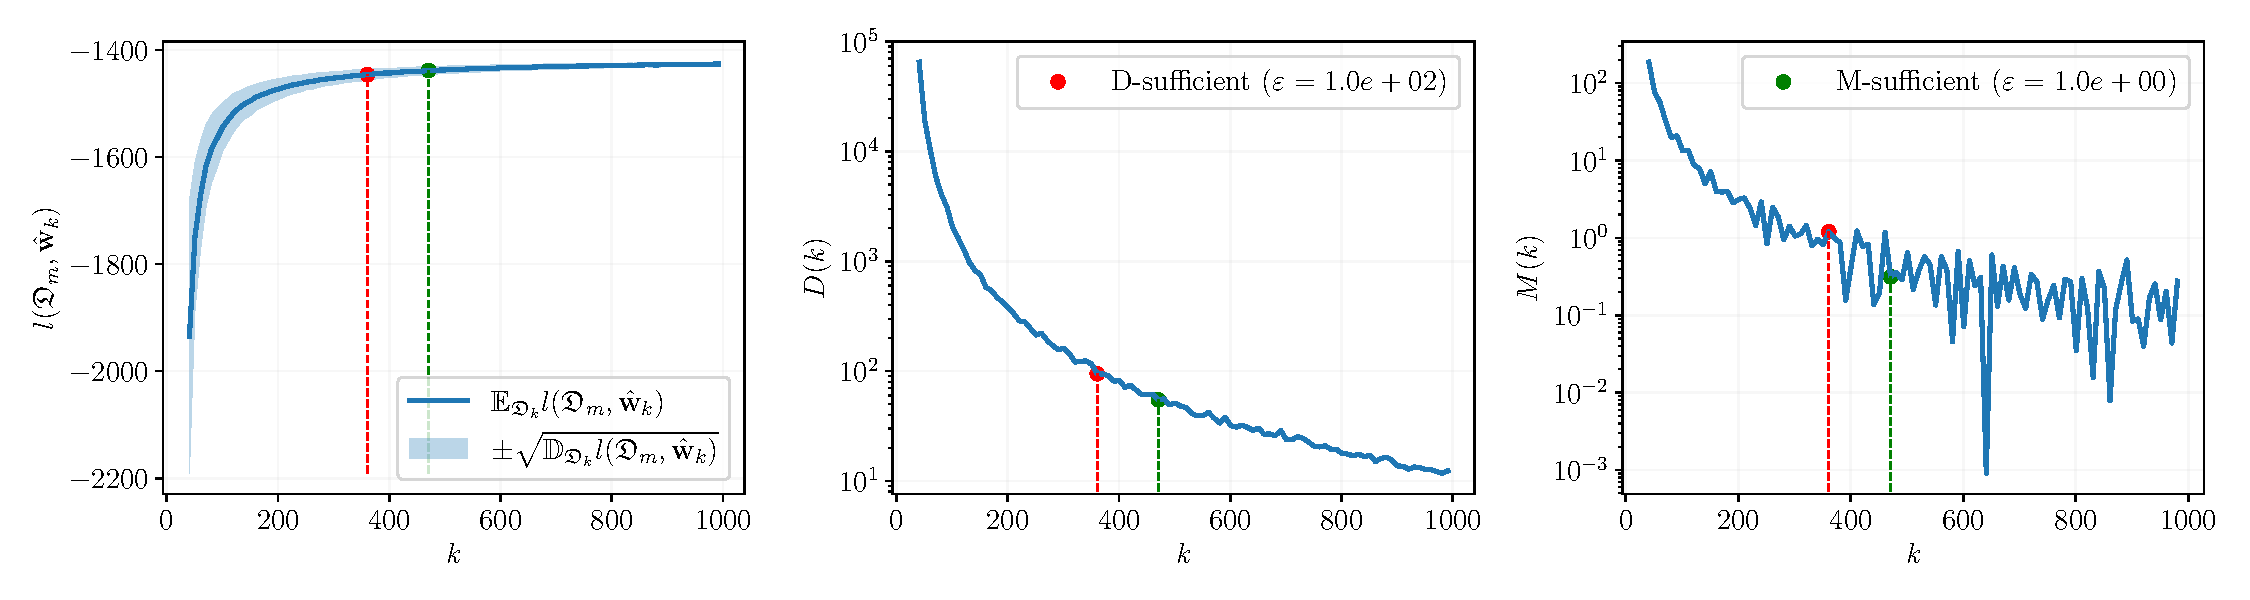
\includegraphics[width=\textwidth]{figures/synthetic-regression-sufficient.pdf}
    \caption{Синтетическая выборка (линейная регрессия) при $m^* \leqslant m$}
    \label{synthetic-regression-sufficient}
\end{figure}

Вторая синтетическая выборка сгенерирована из модели логистической регрессии. Число объектов 1000, число признаков 20. Аналогичные графики приведены на Рис.~\ref{synthetic-classification-sufficient}.

\begin{figure}[h!]
    \centering
    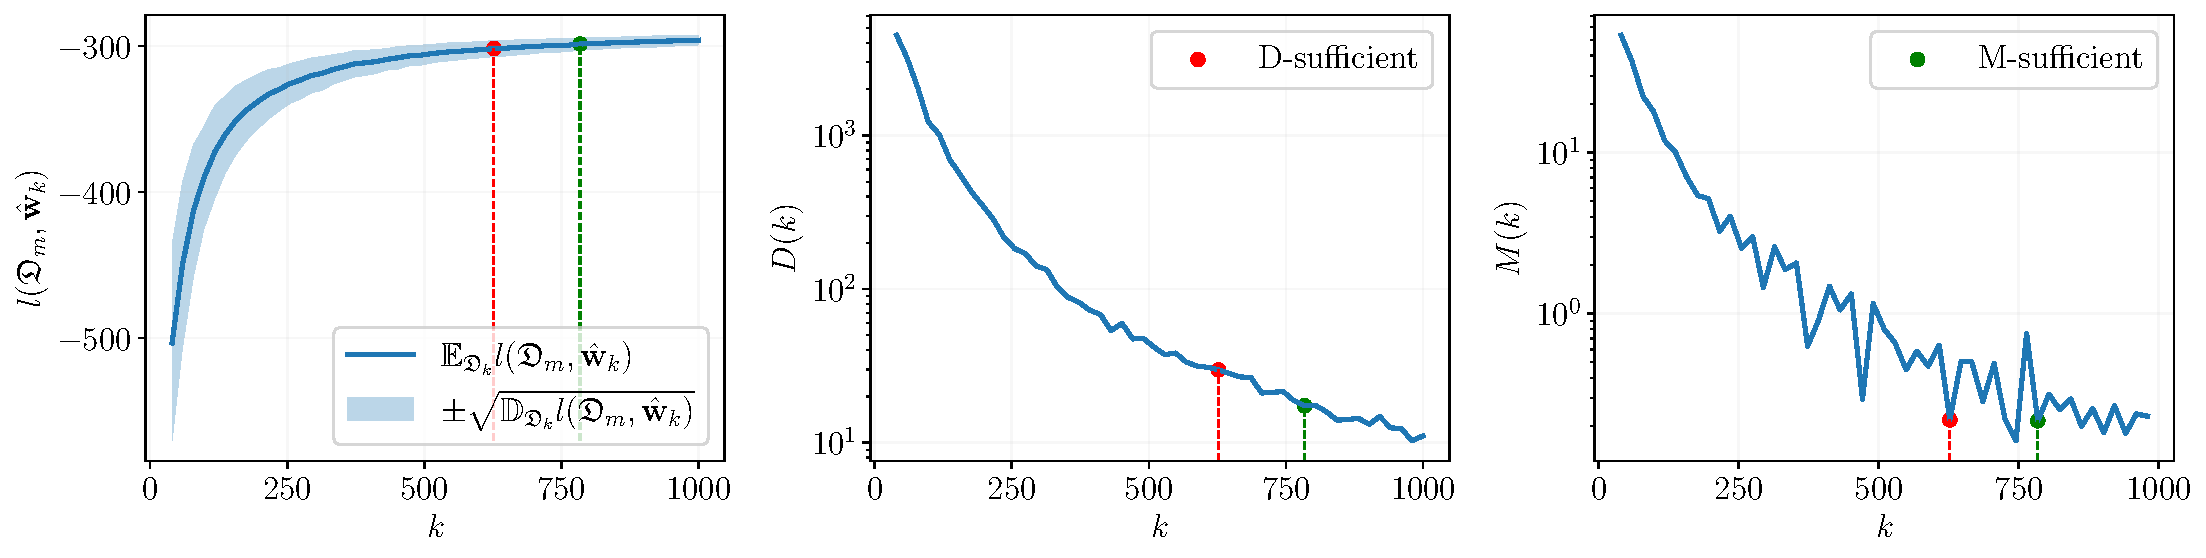
\includegraphics[width=\textwidth]{figures/synthetic-classification-sufficient.pdf}
    \caption{Синтетическая выборка (логистическая регрессия) при $m^* \leqslant m$}
    \label{synthetic-classification-sufficient}
\end{figure}

\subsection{Достаточный размер выборки больше доступного}

Для синтетических выборок проведена аппроксимация функций правдоподобия. Среднее значение и дисперсия аппроксимированы соответственно функциями
\[ \varphi(m) = a_1 - a_2^2 \exp\left( - a_3^2 m \right) - \dfrac{a_4^2}{m^{3/2}} \]
и
\[ \psi(m) = b_1^2 \exp\left( - b_2^2 m \right) + \dfrac{b_3^2}{m^{3/2}}, \]
где $\mathbf{a}$ и $\mathbf{b}$~--- вектора параметров.

Производилось разделение на обучающую и тестовую выборки в соотношении 70:30. Аппроксимация производилась только на обучающей части. Достаточный размер выборки находился в тестовой части. На Рис.~\ref{synthetic-regression-approximation} и Рис.~\ref{synthetic-classification-approximation} представлены истинные и восстановленные зависимости. Там же указаны определенные D-достаточный и M-достаточный размеры выборки.

\begin{figure}[h!]
    \centering
    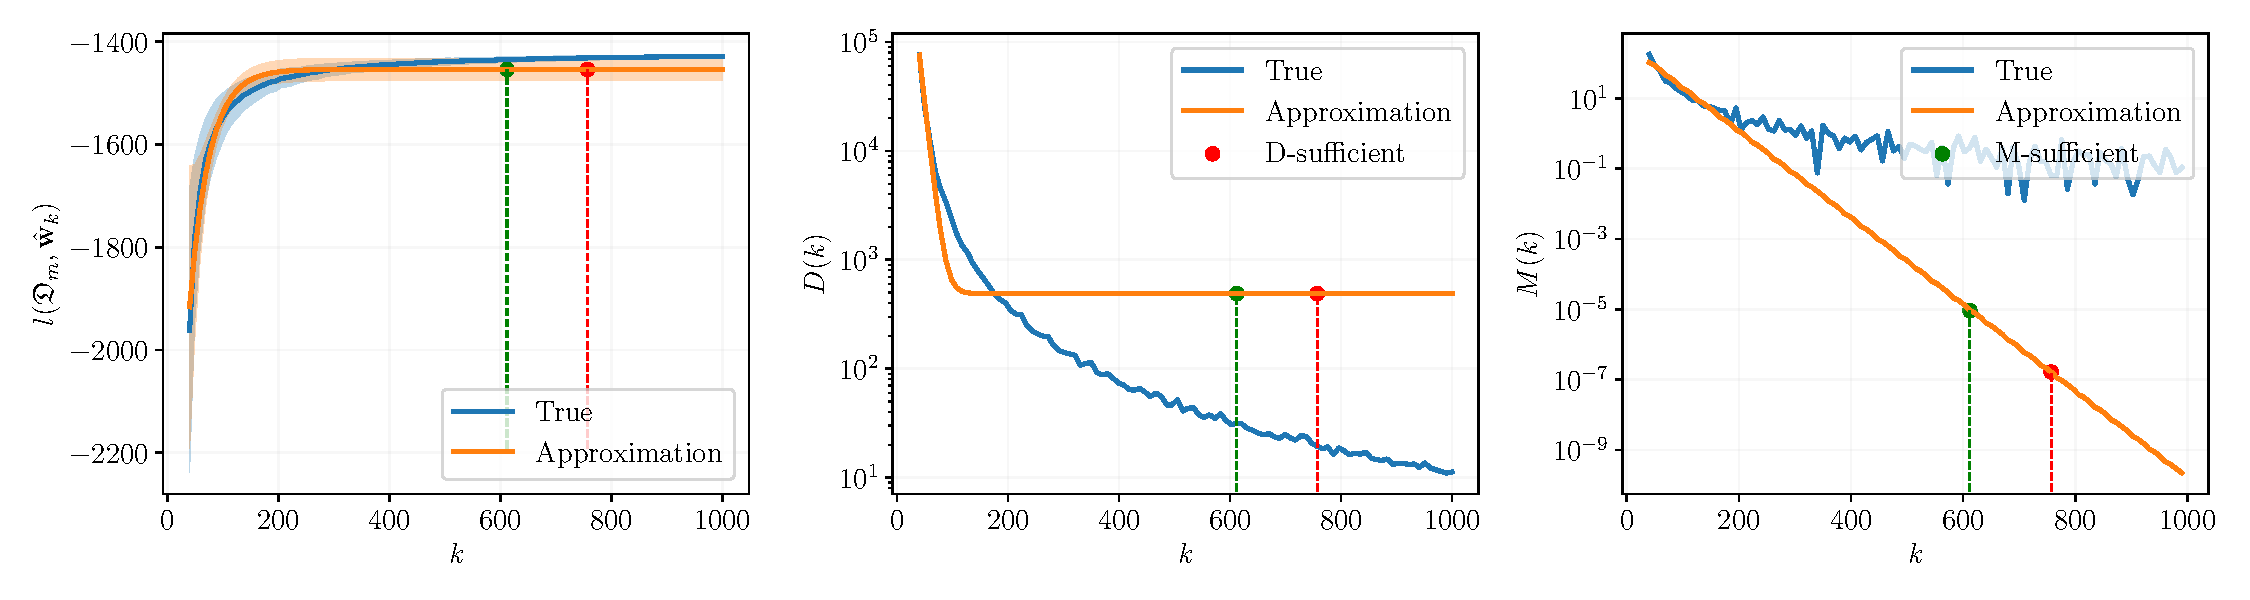
\includegraphics[width=\textwidth]{figures/synthetic-regression-approximation.pdf}
    \caption{Синтетическая выборка (линейная регрессия) при $m^* > m$}
    \label{synthetic-regression-approximation}
\end{figure}

\begin{figure}[h!]
    \centering
    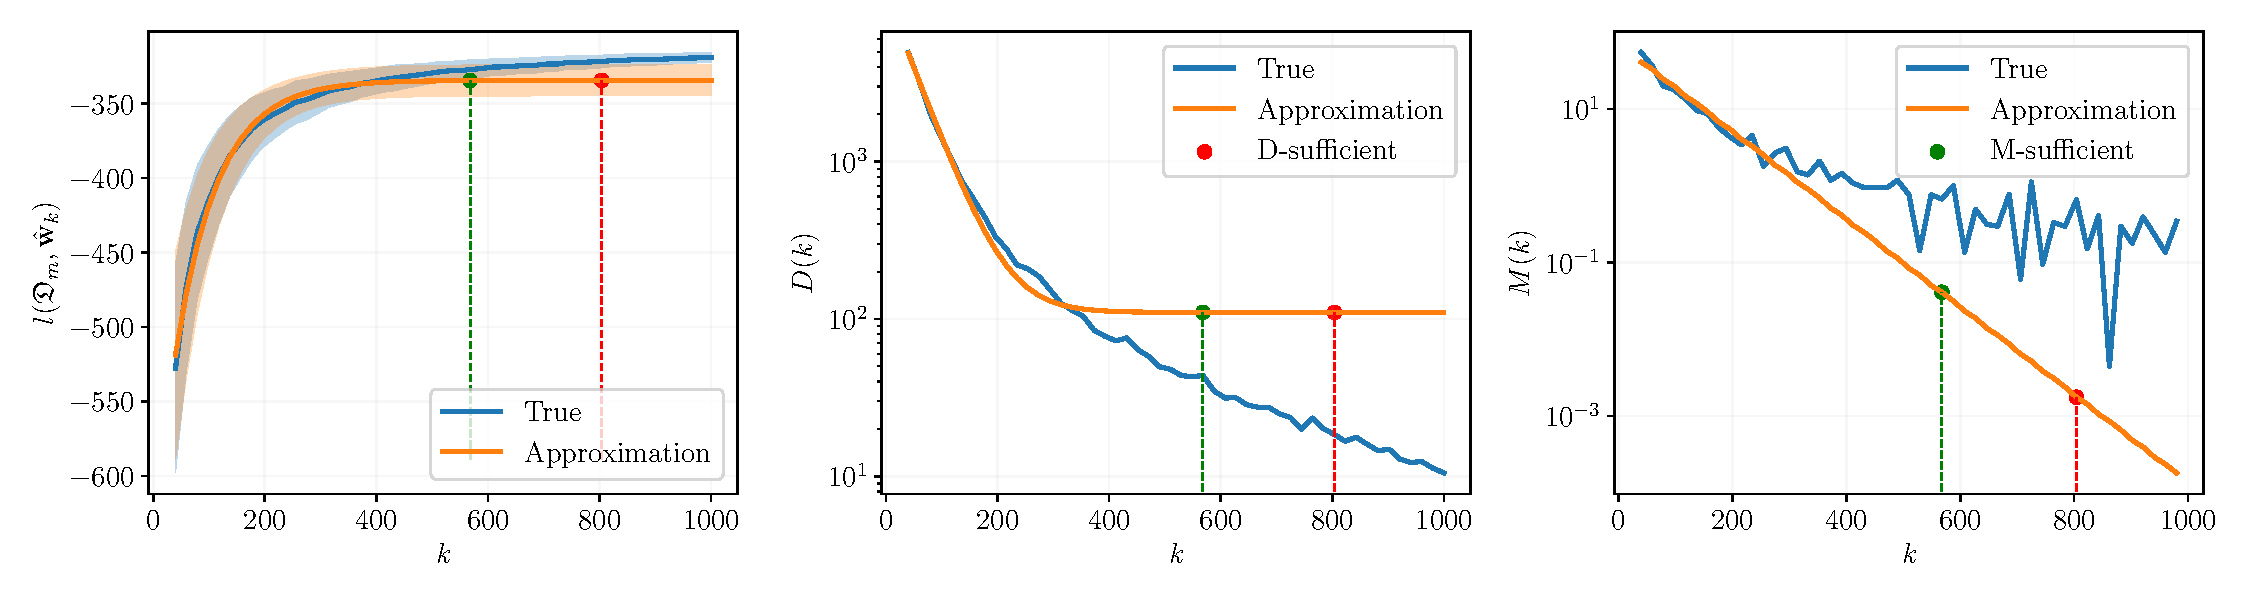
\includegraphics[width=\textwidth]{figures/synthetic-classification-approximation.pdf}
    \caption{Синтетическая выборка (логистическая регрессия) при $m^* > m$}
    \label{synthetic-classification-approximation}
\end{figure}

%%% Заключение
\section{Заключение}

Основные результаты данной работы заключаются в следующем. Предложены способы определения достаточного размера выборки, не использующие распределение параметров модели. Это позволяет применять их для любой модели прогнозирования, будь то линейная регрессия или нейронная сеть. В частном случае доказана корректность такого определения. Проведены вычислительные эксперименты, подтверждающие теоретические выкладки и демонстрирующие работу метода.

%%% Список литературы
\bibliographystyle{abbrv}
\bibliography{references}

\end{document}